\part{Celestial Sphere \&  Asymptotic Flat Spacetime}
\section{Carter-Penrose diagram}
Minkowski时空的度规在球坐标系下可以写为:

\begin{equation}
	ds^2=-dt^2+dr^2+r^2\eqnmarkbox[red]{node}{\left(d\theta^2+\sin^2\theta d\phi^2\right)}
\end{equation}
\annotate[yshift=0.7em]{}{node}{$d{\Omega_2}^2$}
定义retarded和advanced坐标为:
\begin{equation}
	u\equiv t-r,\quad v\equiv t+r
\end{equation}
这个坐标系下度规重写为:
\begin{equation}
	ds^2=-dudv+\frac{(u-v)^2}{4}d{\Omega_2}^2,\quad -\infty<u\leq v <+\infty
\end{equation}
由于时空具有球对称性,所以考虑忽视角向,只考虑径向,那么时空图$t\mbox{-}r$上每一个点代表一个球面,径向光线意味着$u$或$v$是常数。时空的无限远有不同的趋向方式,这也导致了不同的无穷远定义:
\begin{marginfigure}
\begin{center}
	\tikzset{every picture/.style={line width=0.75pt}} %set default line width to 0.75pt        
	
	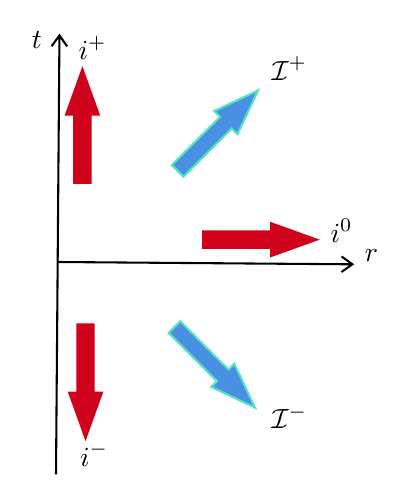
\begin{tikzpicture}[x=0.75pt,y=0.75pt,yscale=-0.75,xscale=0.75]
		%uncomment if require: \path (0,609); %set diagram left start at 0, and has height of 609
		
		%Shape: Axis 2D [id:dp7821872331367214] 
		\draw  (196.6,214.86) -- (385.94,216.34)(197.75,69.29) -- (195.53,351.32) (378.98,211.29) -- (385.94,216.34) -- (378.9,221.29) (192.69,76.25) -- (197.75,69.29) -- (202.69,76.33)  ;
		%Up Arrow [id:dp5623641448201375] 
		\draw  [color={rgb, 255:red, 208; green, 2; blue, 27 }  ,draw opacity=1 ][fill={rgb, 255:red, 208; green, 2; blue, 27 }  ,fill opacity=1 ] (202,120.2) -- (212.5,91) -- (223,120.2) -- (217.75,120.2) -- (217.75,164) -- (207.25,164) -- (207.25,120.2) -- cycle ;
		%Up Arrow [id:dp9355069637780506] 
		\draw  [color={rgb, 255:red, 208; green, 2; blue, 27 }  ,draw opacity=1 ][fill={rgb, 255:red, 208; green, 2; blue, 27 }  ,fill opacity=1 ] (225,298.8) -- (214.5,328) -- (204,298.8) -- (209.25,298.8) -- (209.25,255) -- (219.75,255) -- (219.75,298.8) -- cycle ;
		%Up Arrow [id:dp8020921103254861] 
		\draw  [color={rgb, 255:red, 208; green, 2; blue, 27 }  ,draw opacity=1 ][fill={rgb, 255:red, 208; green, 2; blue, 27 }  ,fill opacity=1 ] (333.8,190) -- (363,200.5) -- (333.8,211) -- (333.8,205.75) -- (290,205.75) -- (290,195.25) -- (333.8,195.25) -- cycle ;
		%Up Arrow [id:dp5136238103533108] 
		\draw  [color={rgb, 255:red, 80; green, 227; blue, 194 }  ,draw opacity=1 ][fill={rgb, 255:red, 74; green, 144; blue, 226 }  ,fill opacity=1 ] (297.24,117.91) -- (325.31,104.69) -- (312.09,132.76) -- (308.37,129.05) -- (277.4,160.02) -- (269.98,152.6) -- (300.95,121.63) -- cycle ;
		%Up Arrow [id:dp5383249274435937] 
		\draw  [color={rgb, 255:red, 80; green, 227; blue, 194 }  ,draw opacity=1 ][fill={rgb, 255:red, 74; green, 144; blue, 226 }  ,fill opacity=1 ] (310.09,280.24) -- (323.31,308.31) -- (295.24,295.09) -- (298.95,291.37) -- (267.98,260.4) -- (275.4,252.98) -- (306.37,283.95) -- cycle ;
		
		% Text Node
		\draw (332,81) node [anchor=north west][inner sep=0.75pt]   [align=left] {$\displaystyle \mathcal{I}^{+}$};
		% Text Node
		\draw (332,305) node [anchor=north west][inner sep=0.75pt]   [align=left] {$\displaystyle \mathcal{I}^{-}$};
		% Text Node
		\draw (208,68) node [anchor=north west][inner sep=0.75pt]   [align=left] {$\displaystyle i^{+}$};
		% Text Node
		\draw (209,329) node [anchor=north west][inner sep=0.75pt]   [align=left] {$\displaystyle i^{-}$};
		% Text Node
		\draw (178,65) node [anchor=north west][inner sep=0.75pt]   [align=left] {$\displaystyle t$};
		% Text Node
		\draw (370,185) node [anchor=north west][inner sep=0.75pt]   [align=left] {$\displaystyle i^{0}$};
		% Text Node
		\draw (392,205) node [anchor=north west][inner sep=0.75pt]   [align=left] {$\displaystyle r$};
	\end{tikzpicture}
\end{center}
\caption{共形无穷远定义}
\end{marginfigure}
\begin{itemize}
	\item[$i^+$]:类时未来无穷远,$r$一定,$t\to+\infty$;
	\item[$i^-$]:类时过去无穷远,$r$一定,$t\to-\infty$;
	\item[$i^0$]:类空无穷远,$t$一定,$r\to+\infty$;
	\item[$\mathcal{I}^+$]:类光未来无穷远,$u$一定,$r\to+\infty$;
	\item[$\mathcal{I}^-$]:类光过去无穷远,$v$一定,$r\to+\infty$;
\end{itemize}
这五个无穷远合称为\textbf{共形无穷远}。

但是无穷远还是一个靠想象的概念,无法在这样的图中表现出来,继续考虑坐标变换,变到所谓光锥坐标:
\begin{equation}
	U\equiv\arctan u ,\quad V\equiv\arctan v
\end{equation}
度规在光锥坐标下变为:
\begin{equation}
	ds^2=\frac{1}{4\cos^2U\cos^2V}\cdot\left(-4dUdV+\sin^2(V-U)d{\Omega_2}^2\right),\quad -\frac{\pi}{2}<U\leq V<\frac{\pi}{2}
\end{equation}
现在我们牺牲对距离的精确描述,考虑Weyl变换之后,丢掉共形因子后的度规:
\begin{equation}\label{eq:15.6}
	\tilde{ds}^2=-4dUdV+\sin^2(V-U)d{\Omega_2}^2
\end{equation}
这样消去了在$\pm\frac{\pi}{2}$处的坐标奇性,我们称之为\textbf{共形紧化}。可以证明\cite{blau},两个相差共形变换的度规具有如下性质:
\begin{itemize}
	\item[1.] 由于$\tilde{ds}^2\iff ds^2=0$,所以光锥不变,即时空因果结构不发生改变;
	\item[2.] 向量场的类时、类空和类光性质不变;
	\item[3.] 类时和类空曲线还是类时或者类空的,但是类时或者类空测地线不一定仍是测地线,但是类光测地线依然是类光测地线。
\end{itemize}
从这个意义上看,如果我们只关注时空的因果结构,完全可以考虑共形紧化之后的度规,重点是共形紧化后坐标变成有限区间内取值,这使得我们有希望在时空图上表现出共形无限远。继续对\ref{eq:15.6}做变换:
\begin{equation}
	T=U+V,\quad R=U-V,\text{overall:}t\pm r=\tan\frac{1}{2}\left(T\pm R\right)
\end{equation}
度规变为:
\begin{equation}
	\tilde{ds}^2=-dT^2+dR^2+\sin^2Rd{\Omega_2}^2,\quad-\pi<T\leq R<\pi
\end{equation}
最后一项角向不用在意\sn{坐标变换的时候我们只是把$r,t$进行变换,没有将他们与角向坐标混合},现在整个时空图是一个有限大小的图,其上面的每一点表示一个球面(除了$i^0$),而且共形无限远以边界的形式表现出来:
\begin{figure}[H]
	\centering
	\includegraphics[width=0.618\linewidth]{figs/cover.pdf}
	\caption{Minkowski时空彭罗斯图}
\end{figure}
这种类光测地线都是$45^\circ$斜线,而且能表示共形无限远的图称为彭罗斯图。这个图还有另一种更常用的画法,注意到上面的图
\begin{figure}[H]
	\centering
	\includegraphics[width=0.618\linewidth]{figs/cover.pdf}
	\caption{Minkowski时空彭罗斯图的另一种形式}
\end{figure}
\section{Conformal infinity}
\section{Asymptotic flat spacetime}
